% Chapter Template

\chapter{M\'etodos} % Main chapter title

\label{Chapter3} % Change X to a consecutive number; for referencing this chapter elsewhere, use \ref{ChapterX}

%----------------------------------------------------------------------------------------
%	SECTION 1
%----------------------------------------------------------------------------------------

\section{Descripci\'on general}

Para la obtenci\'on de una im\'agen que es utilizada por personal de la salud para la detecci\'on de una enfermedad o la realizaci\'on de un diagnostico prec\'oz respecto a un afecci\'on que sufre el paciente, es necesario realizar un preprocesamiento de las imagenes de fondo de ojo teniendo en cuenta que la misma es de suma importancia para la atenci\'on y posible tratamiento de una persona con problemas visuales severos o no.

Con el fin de generar una im\'agen que permita al Medico proveer ayuda en su diagn\'ostico, es necesario preprocesar la captura de fondo de ojo y de esta forma acercarle una im\'agen mas clara que la obtenida por la herramienta utilizada en la captura de la misma.




%-----------------------------------
%	SECTION 2
%-----------------------------------
\section{Preprocesamiento}

El preprocesamiento digital de im\'agenes permite mejorar distintos aspectos de la misma, de este modo se puede determinar con mayor efectividad el diagn\'ostico correspondiente.

En este sentido, esta etapa de preprocesamiento busca mejorar algunos de los siguientes:

\begin{itemize}
	\item[$*$] Suavizar la im\'agen:  reducir la cantidad de variaciones de intensidad entre píxeles vecinos.					\item[$*$] Eliminar ruido: eliminar aquellos píxeles cuyo nivel de intensidad es muy diferente al de sus vecinos y cuyo origen puede estar tanto en el proceso de adquisición de la imagen como en el de transmisión.
	\item[$*$] Realzar bordes: destacar los bordes que se localizan en una imagen.
	\item[$*$] Detectar bordes: detectar los píxeles donde se produce un cambio brusco en la función intensidad.
\end{itemize}

En el desarrollo inicial de este trabajo se utilizaron diferentes m\'etodos para determinar el mejor preprocesamiento a utilizar en los sets de im\'agenes propuestos, HRF, ARIA y DRIVE. Los mismos contienen im\'agenes con diferentes enfermedades, tales como, retinopat\'ia diab\'etica, edema macular asociado a la edad e im\'agenes sanas entre otras. 

En primer lugar, se determinaron los algoritmos a utilizar para mejorar el preprocesamiento de las im\'agenes, es decir, disminuir los efectos secundarios que se generan en la captura de im\'agenes de fondo de ojo como los nombrados anteriormente. 

Para la eliminaci\'on o extracci\'on del ruido se tuvieron en cuenta dos algoritmos: filtro de Difusi\'on Anisotr\'opica y filtro de  Coherencia.\\

El filtro de Difusi\'on anisotr\'opica es una técnica destinada a reducir el ruido de una imagen sin necesidad de retirar las piezas importantes del contenido de la imagen, por lo general los bordes, líneas u otros detalles que son importantes para la interpretación de la imagen el modelo de difusión anisotrópico asemeja el proceso que crea un espacio de escala, donde una imagen genera una familia parametrizada de forma sucesiva cada vez más borrosas de imágenes, basadas en un proceso de difusión(Ref WIKIPEDIA).\\

El filtro de Coherencia ...This function COHERENCEFILTER will perform Anisotropic Diffusion of a 2D gray/color image or 3D image volume, Which will reduce the noise in an image while preserving the region edges, and will smooth along
the image edges removing gaps due to noise.\\

Para la eliminaci\'on o extracci\'on del fondo se tuvieron en cuenta tres filtros denominados de paso bajo, el filtro de mediana, el filtro de media y el filtro gaussiano. 

El proceso de filtrado consiste en la aplicación a cada uno de los pixels de la imagen de una matriz de filtrado de tamaño N x N (generalmente de 3x3 aunque puede ser mayor) compuesta por números enteros y que genera un nuevo valor mediante una función del valor original y los de los pixels circundantes. El resultado final se divide entre un escalar, generalmente la suma de los coeficientes de ponderación. Los filtros se pueden expresar mediante una ecuación (6.1)

\begin{displaymath}
N D'_i,_j=\frac{ND_{i-1},_{j-1} + ND_{i},_{j-1} + ND_{i+1},_{j-1} + ND_{i-1},_{j} + ND_{i},_{j} + ND_{i+1},_{j} + ND_{i-1},_{j+1} + ND_{i-1},_{j+1} + ND_{i-1},_{j+1}}{9}
\end{displaymath}

donde i y j representan la fila y la columna de cada pixel, N \[D_{i;j}\] su Nivel Digital y ND 0 i;j el Nivel Digital obtenido tras hacer el filtrado.\\

El objetivo de estos consiste en suavizar la im\'agen, son útiles cuando se supone que la imagen tiene gran cantidad de ruido y se quiere eliminar. También pueden utilizarse para resaltar la información correspondiente a una determinada escala (tamaño de la matriz de filtrado); 


\begin{itemize}
	\item[$*$] Filtro de la media, asigna al pixel central la media de todos los pixeles incluidos en la ventana. La matriz de filtrado estaría compuesta por unos y el divisor sería el número total de elementos en la matriz.					\item[$*$] Filtro de la mediana tiene la ventaja de que el valor final del pixel es un valor real presente en la imagen y no un promedio, de este modo se reduce el efecto borroso que tienen las imagenes que han sufrido un filtro de media. Además el filtro de la mediana es menos sensible a valores exremos. El incoveniente es que resulta más complejo de calcular ya que hay que ordenar los diferentes valores que aparecen en los pixeles incluidos en la ventana y determinar cual es el valor central.
	\item[$*$]Filtros gaussianos. Simulan una distribución gaussiana bivariante. El valor máximo aparece en el pixel central y disminuye hacia los extremos tanto más rápido cuanto menor sea el parámetro de desviación típica s. El resultado será un conjunto de valores entre 0 y 1. Para transformar la matriz a una matriz de números enteros se divide toda la matriz por el menor de los valores obtenidos. La ecuación para calcularla es:
\end{itemize}

(REF pdf Tecnicas de Filtrado -tema06.pdf)\\

IMAGENES DE MATRICES PARA MEDIA, MEDIANA Y GAUSSIANO\\

%\begin{figure*}[t!]
%    \centering
%    \begin{subfigure}[t]{0.5\textwidth}
%        \centering
%        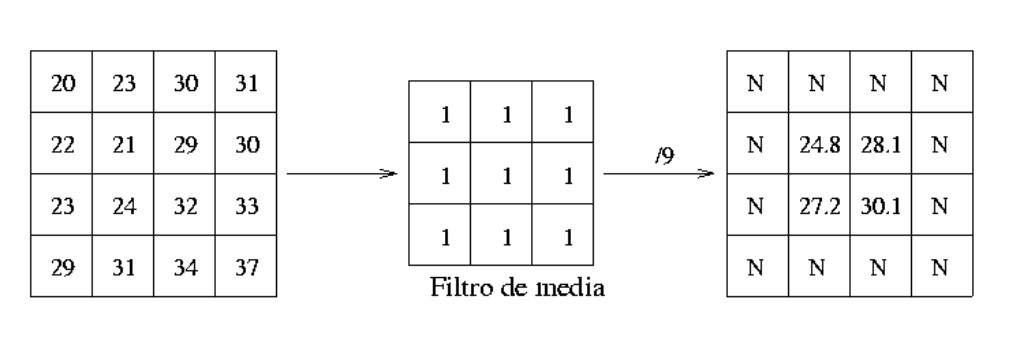
\includegraphics[height=1.2in]{media}
%        \caption{Lorem ipsum}
%    \end{subfigure}%
%    ~ 
%    \begin{subfigure}[t]{0.5\textwidth}
%        \centering
%        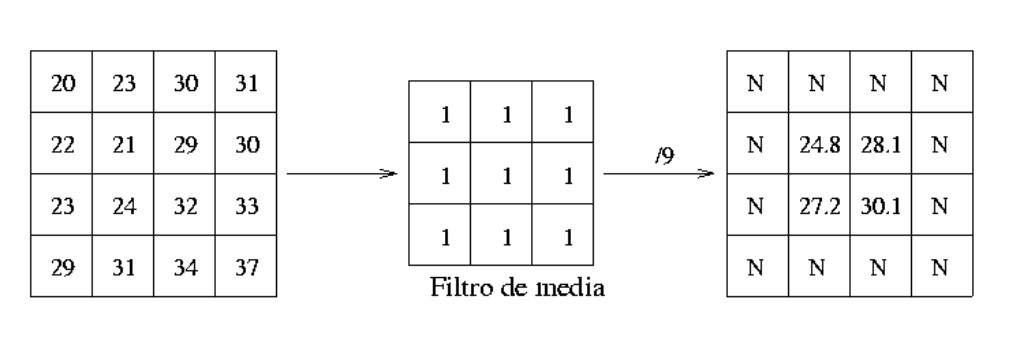
\includegraphics[height=1.2in]{media}
%        \caption{Lorem ipsum, lorem ipsum,Lorem ipsum, lorem ipsum,Lorem ipsum}
%    \end{subfigure}
%    \caption{Caption place holder}
%\end{figure*}



Con los métodos de filtrado definidos y analizados teniendo en cuenta sus ventajas y desventajas, se realizaron cuatro pipelines para determinar cual de estos es el mejor para utilizar en los sets de im\'agenes propuestos.

\begin{itemize}
	    \item Pipeline 1 -> Extracci\'on de fondo  +  Realce  +  Extracci\'on de ruido
		\item Pipeline 2 -> Realce +  Extracci\'on de ruido
		\item Pipeline 3 -> Realce +  Extracci\'on de fondo
		\item Pipeline 4 -> Realce  + Extracci\'on de fondo   +  Extracci\'on de ruido
\end{itemize}


Inicialmente se obtiene el canal verde de la im\'agen, el cual permite observar de manera mas clara los vasos sangu\'ineos de la misma. Una vez realizdo esto, se procesan las im\'agenes por los pipelines nombrados anteriormente.
A continuaci\'on se describe cada etapa, detallando de que se encarga cada una de ellas:

\begin{itemize}
	\item Extracci\'on de fondo: para esta etapa se realizaron pruebas con los tres filtros nombrados mas arriba. El objetivo de  esta etapa consiste en suavizar la im\'agen, para esto calculamos el fondo de la imagen, luego le restamos a la imagen original este fondo y de esta manera podemos remover el efecto de bias causado por la modalidad de captura de la imagen. Finalmente se convierte la imagen a double para tener mayor precisión en las próximas etapas.\\
Codigo de media, mediana y gaussiano\\
	\item Extracción de ruido:  Esta etapa consiste en aplicar un filtro que sea capaz de eliminar el ruido provocado por el método de captura o procesamiento de la  imagen, como así también el ruido ocasionado por la suciedad del lente, partículas en suspensión, etc. 
Para esta etapa se aplicaron los filtros de difusión anisotropica y filtro anisotrópico de realce de coherencia con el esquema de difusión isotrópica de Perona y Malik.
	\item Realce: Esta función realiza la Ecualización Adaptativa de la imagen permitiendo percibir detalles cuando el fondo no es homogéneo. Es decir, que el realce pretende mejorar el contraste de una imagen, haciendo que "los píxeles claros se aclaren más" y "los píxeles oscuros se oscurezcan". 
\end{itemize}

Para determinar cual de los pipeline es el que permite obtener el mejor preprocesado de las imágenes, se fueron variando los parametros correspondientes a cada filtro y analizando el resultado del mismo, teniendo en cuenta el valor de área promedio bajo la curva obtenido.

El resultado se logra comparando la imágen preprocesada con la imágen del ground true correspondinte. Esta comparación se realza con el método vlroc provisto por Matlab,  herramienta de software matemático que ofrece un entorno de desarrollo integrado (IDE) con un lenguaje de programación propio (lenguaje M). 

El área bajo la curva, también llamada región de interés, devuelve un valor acotado entre 0 y 1, siendo 1 el mejor y mayor valor alcanzable. Este valor de área es un resultado promedio, ya que se procesan todas las imágenes pertenecientes a un mismo dataset y finalmente se obtiene este valor que luego es utilizado para el análisis de la imágen.\\

Para cada conjunto de imágenes se aplicaron los pipelines descritos anteriormente.\\
En cuanto a la variación de parámetros en la extracción de fondo, se realizó una busqueda exhaustiva para obtener la mejor ventana para cada uno de los sets. Para esto se realizó una iteración sobre el total de imágenes para distintos tamaños de ventanas y finalmente se encontró el óptimo para cada uno. Por razones de costo computacional, las iteraciones para la obtención de la mejor ventana, se realizó con tamaños de ventanas en el rango de 3 a 400. Inicialmente se iteró en este rango con saltos de 20 pasos, para así poder encontrar la curva aproximada con el valor máximo y luego disminuir el rango como así también los saltos.\\

Para la extracción de ruido se utilizó un procedimiento similar para obtener el mejor numero de iteraciones para un mejor resultado. A diferencia del procedimiento de extracción de fondo, este es un proceso computacionalmente costoso, encontrandose el filtro de Coherencia muy por encima del filtro de difusión anisotrócipa.
En el filtro de coherencia, se realizaron iteraciones de hasta 105, pero luego se disminuyo a 50 iteraciones debido a que en relación costo-beneficio no hay mejoras sustanciales para numeros altos de iteraciones.

Tambien se realizaron pruebas, para determinar el valor del parámetro kappa, se observo que este parámetro entrega su mejor resultado cuando es igual a dos.


\subsection{Dataset ARIA}

A continuación se muestran resultados logrados en el preprocesado de las imágenes para la obtención del tamaño de ventana óptimo para el dataset Aria.\\

Extracción de fondo
\begin{itemize}
	\item[$*$]Mediana 
\end{itemize}
Se realiz\'o una iteraci\'on con el tamaño de ventana variando desde 3 hasta 200, con pasos de a 10. De esta forma se obtuvo el siguiente resultado(\ref{fig:MedianaRangoGrande})\\

\begin{figure}[H]
	{
	\centering
	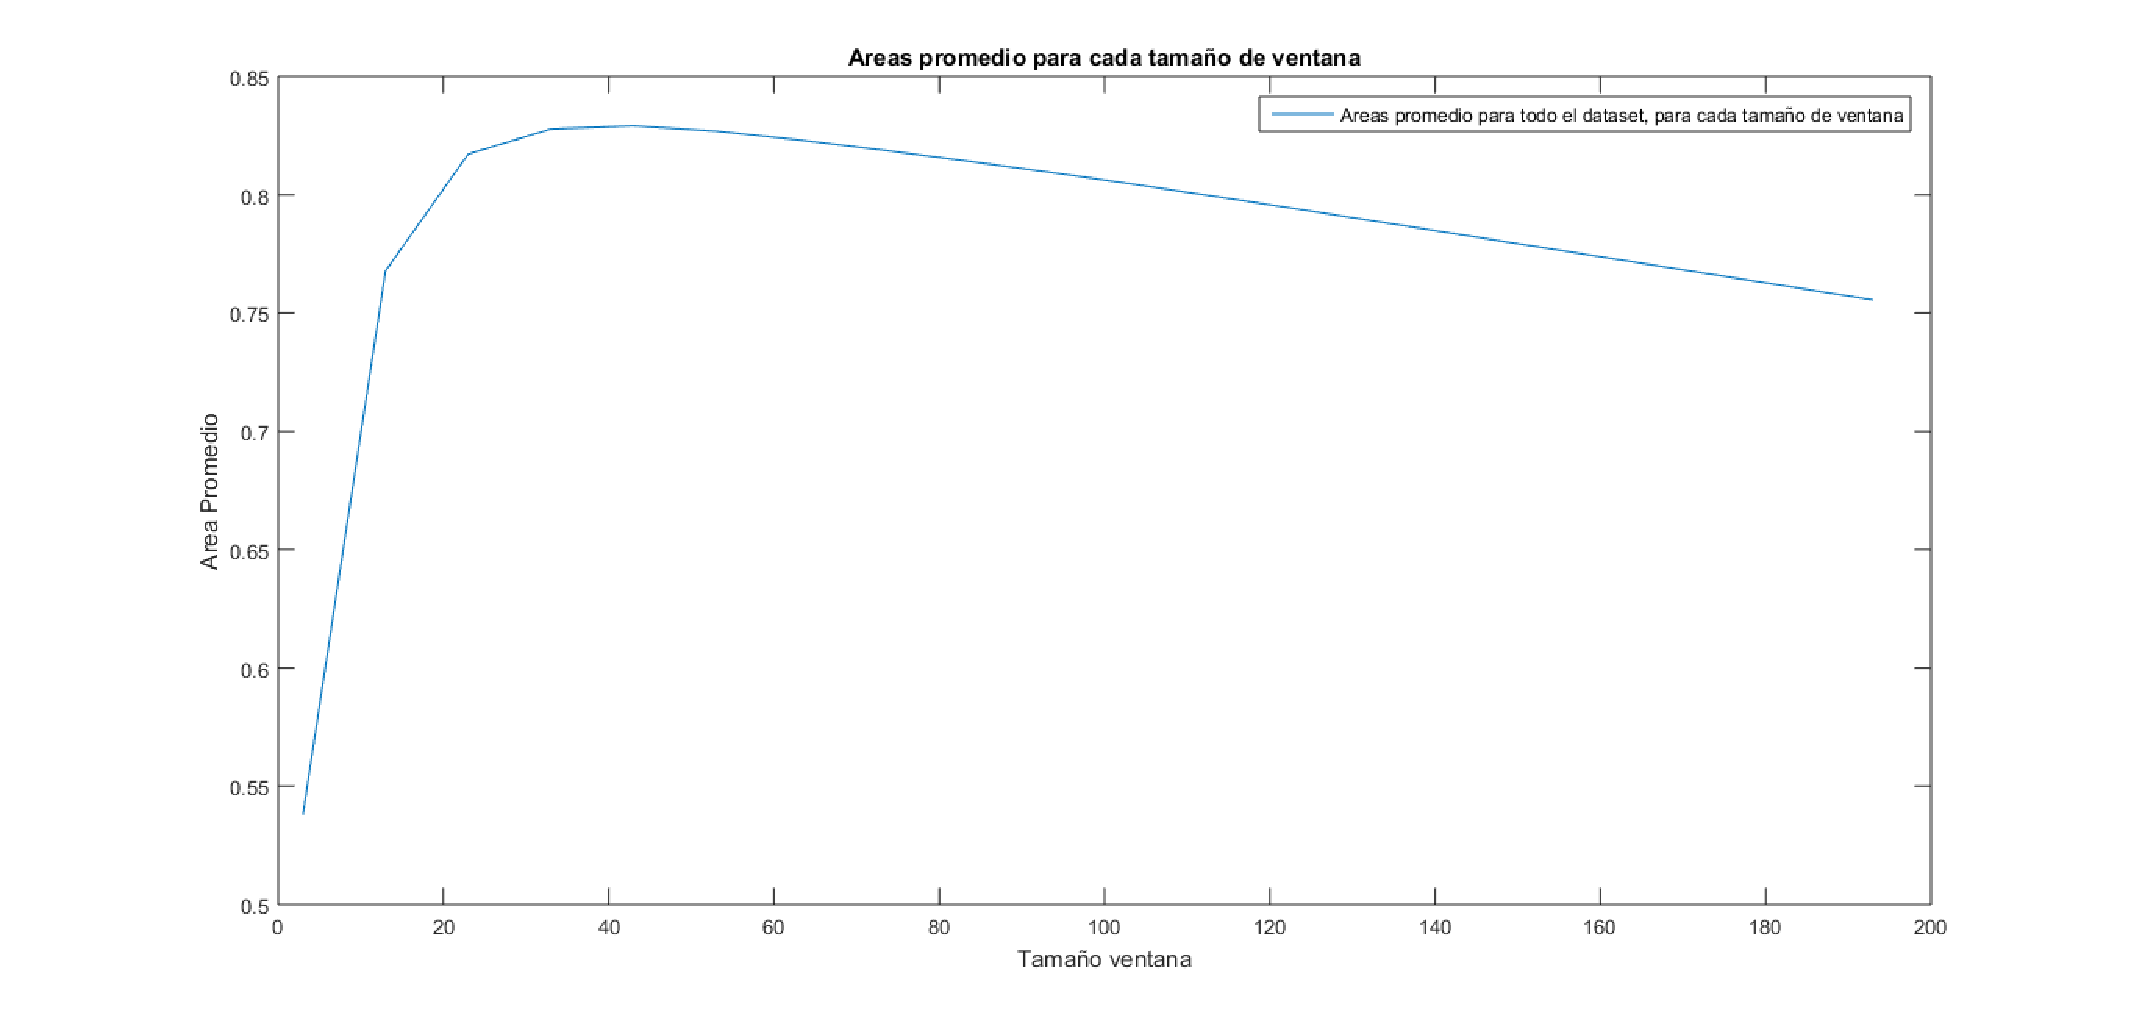
\includegraphics[width=1\textwidth]{Figures/MedianaRangoGrande}
	\caption[Ventana Mediana 0-200]{\'Areas promedio para diferentes tamaños de ventana, en el rango 0-200.}
	\label{fig:MedianaRangoGrande}
	}
\end{figure}	

De la im\'agen anterior se puede ver que el valor m\'aximo se encuentre en un rango mas chico, por esta  raz\'on se realiza otra iteraci\'on con un tamaño de ventanas variando de 15 a 60. De este modo, mirando el gr\'afico obtenido (\ref{fig:MedianaRangoChico}) se puede observar que  el mejor tama\~no de ventana es 41 ya que es el punto m\'aximo de la par\'abola con un valor de \'area bajo la curva de 0.8292.

\begin{figure}[H]
	{
	\centering
	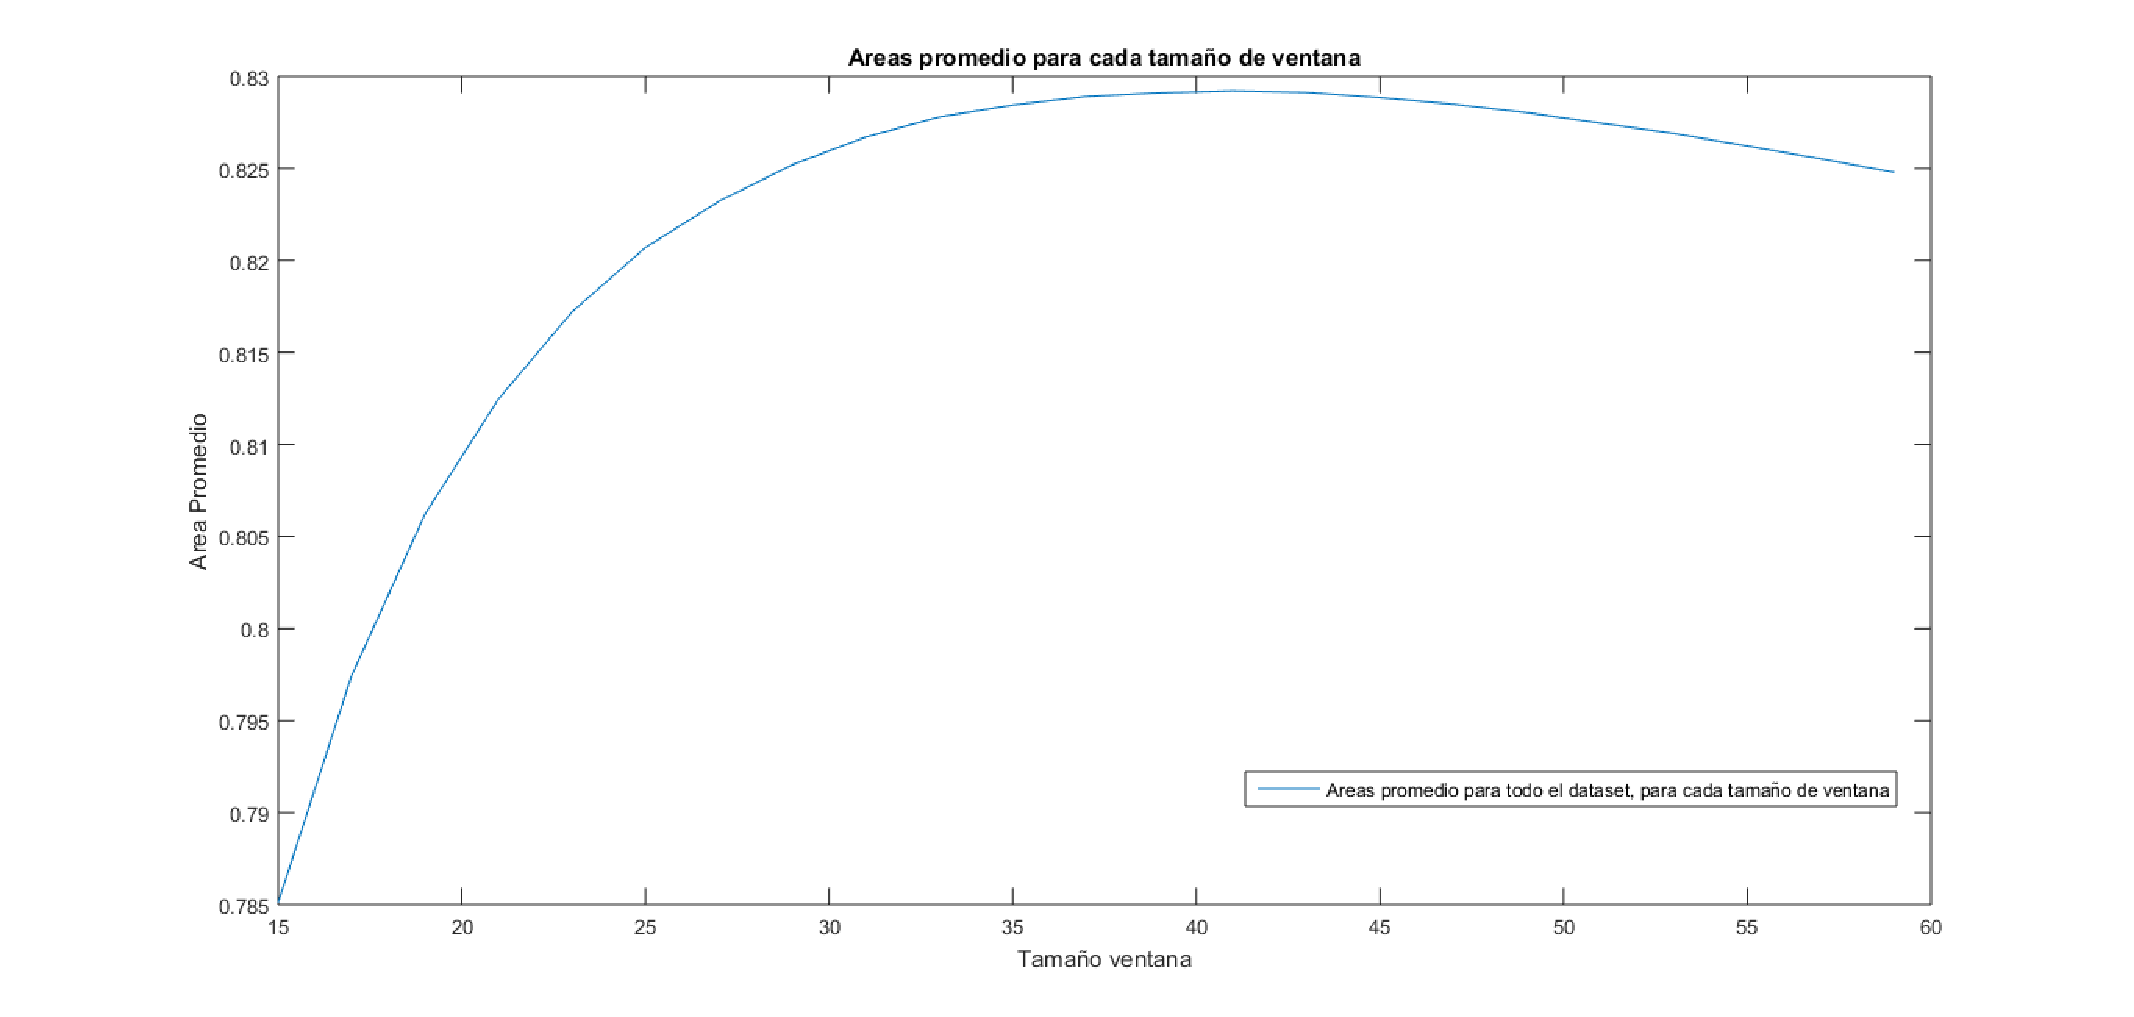
\includegraphics[width=1\textwidth]{Figures/MedianaRangoChico}
	\caption[Ventana Mediana 15-60]{\'Areas promedio para diferentes tamaños de ventana, en el rango 15-60.}
	\label{fig:MedianaRangoChico}
	}
\end{figure}	

\begin{itemize}
	\item[$*$]Media
\end{itemize}

Para la b\'usqueda de la ventana \'optima en la media, se realiz\'o en primer lugar una iteraci\'on en un rango desde 7 hasta 550 con pasos de a 20 obteni\'endose el siguiente resultado (\ref{fig:MediaRangoGrande}):

\begin{figure}[H]
	{
	\centering
	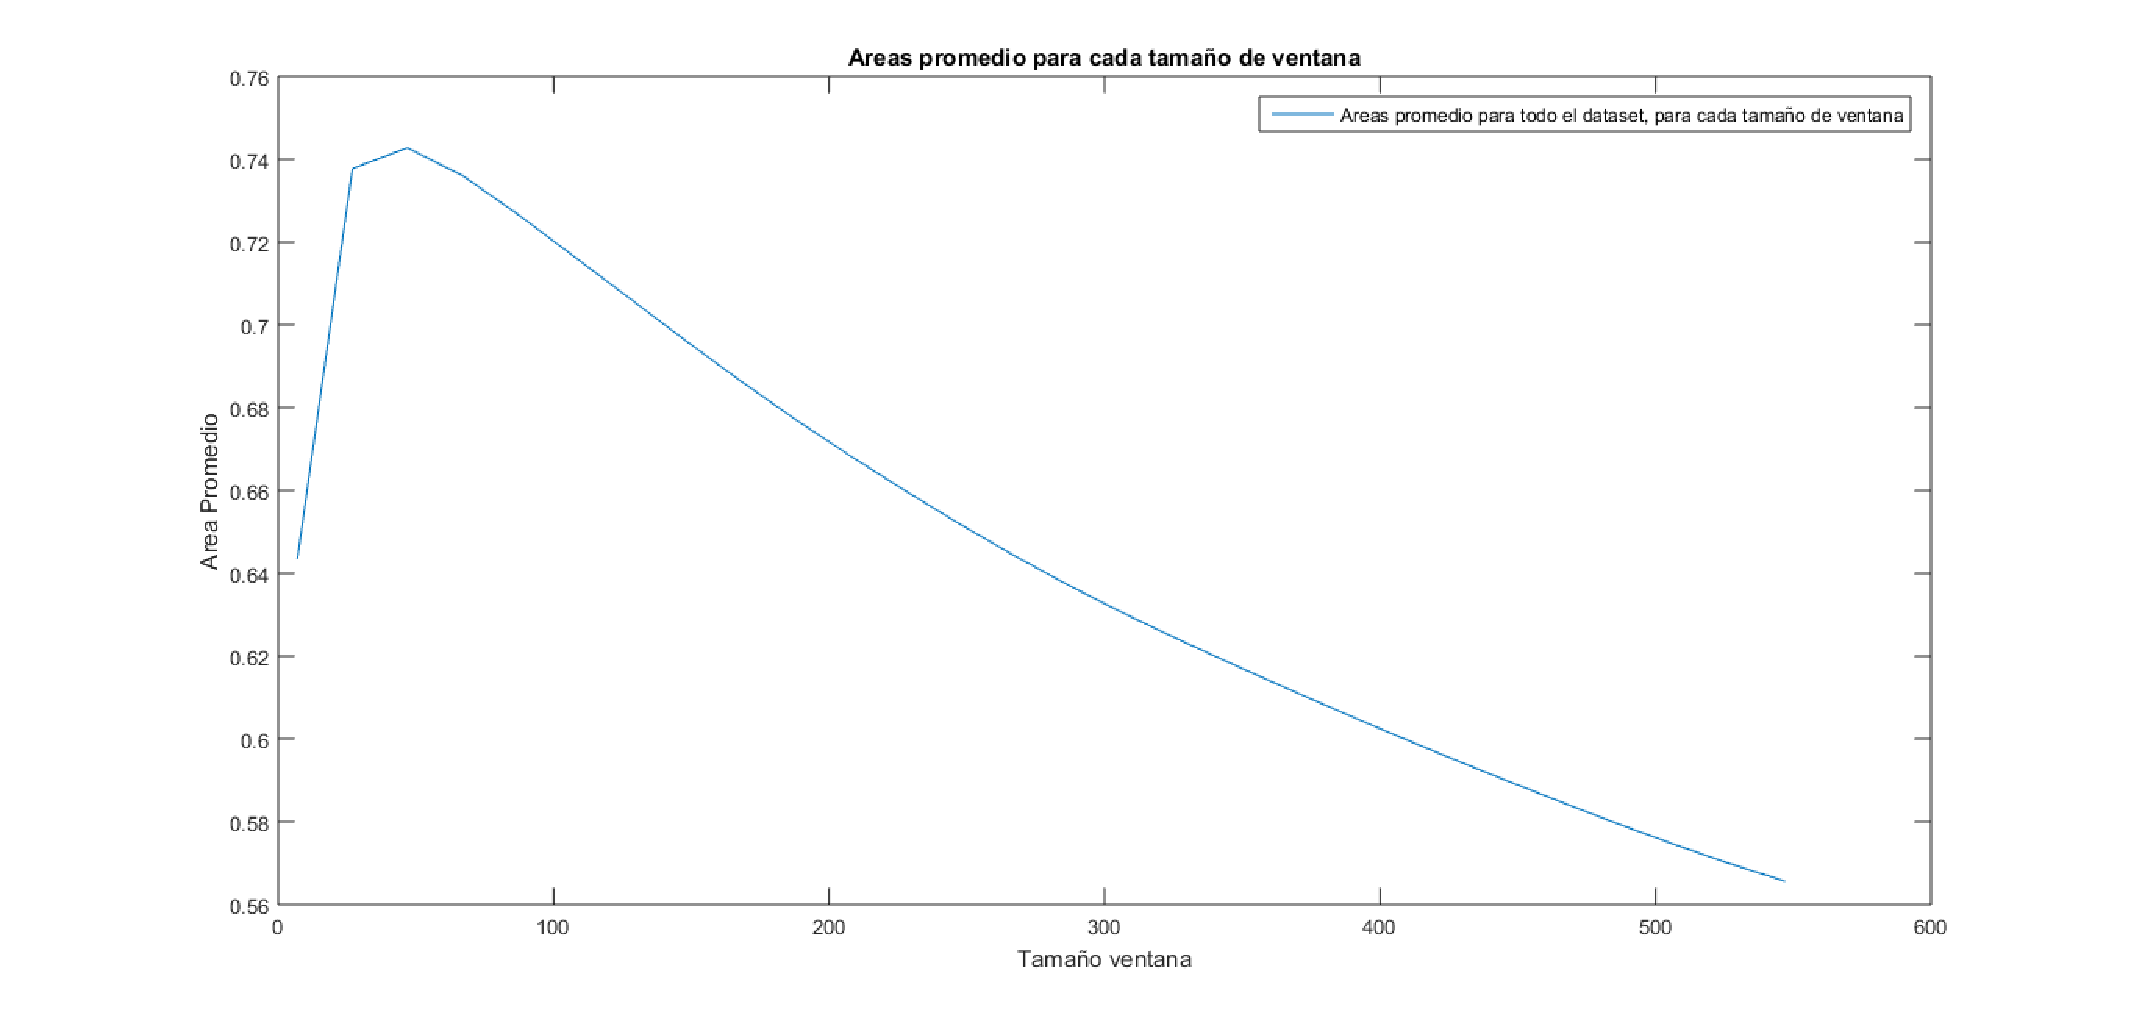
\includegraphics[width=1\textwidth]{Figures/MediaRangoGrande}
	\caption[Ventana Media 7-550]{\'Areas promedio para diferentes tama\~nos de ventana, en el rango 7-550.}
	\label{fig:MediaRangoGrande}
	}
\end{figure}

De la im\'agen anterior se puede ver que el valor m\'aximo se encuentra en un rango mas chico, por esta  raz\'on se realiza otra iteraci\'on con un tama\~no de ventana variando de 15 a 80. De este modo, mirando el gr\'afico obtenido  (\ref{fig:MediaRangoChico}) se puede observar que  el mejor tama\~no de ventana es 41 ya que es el punto m\'aximo de la par\'abola con un valor de \'area bajo la curva de 0.7435.

\begin{figure}[H]
	{
	\centering
	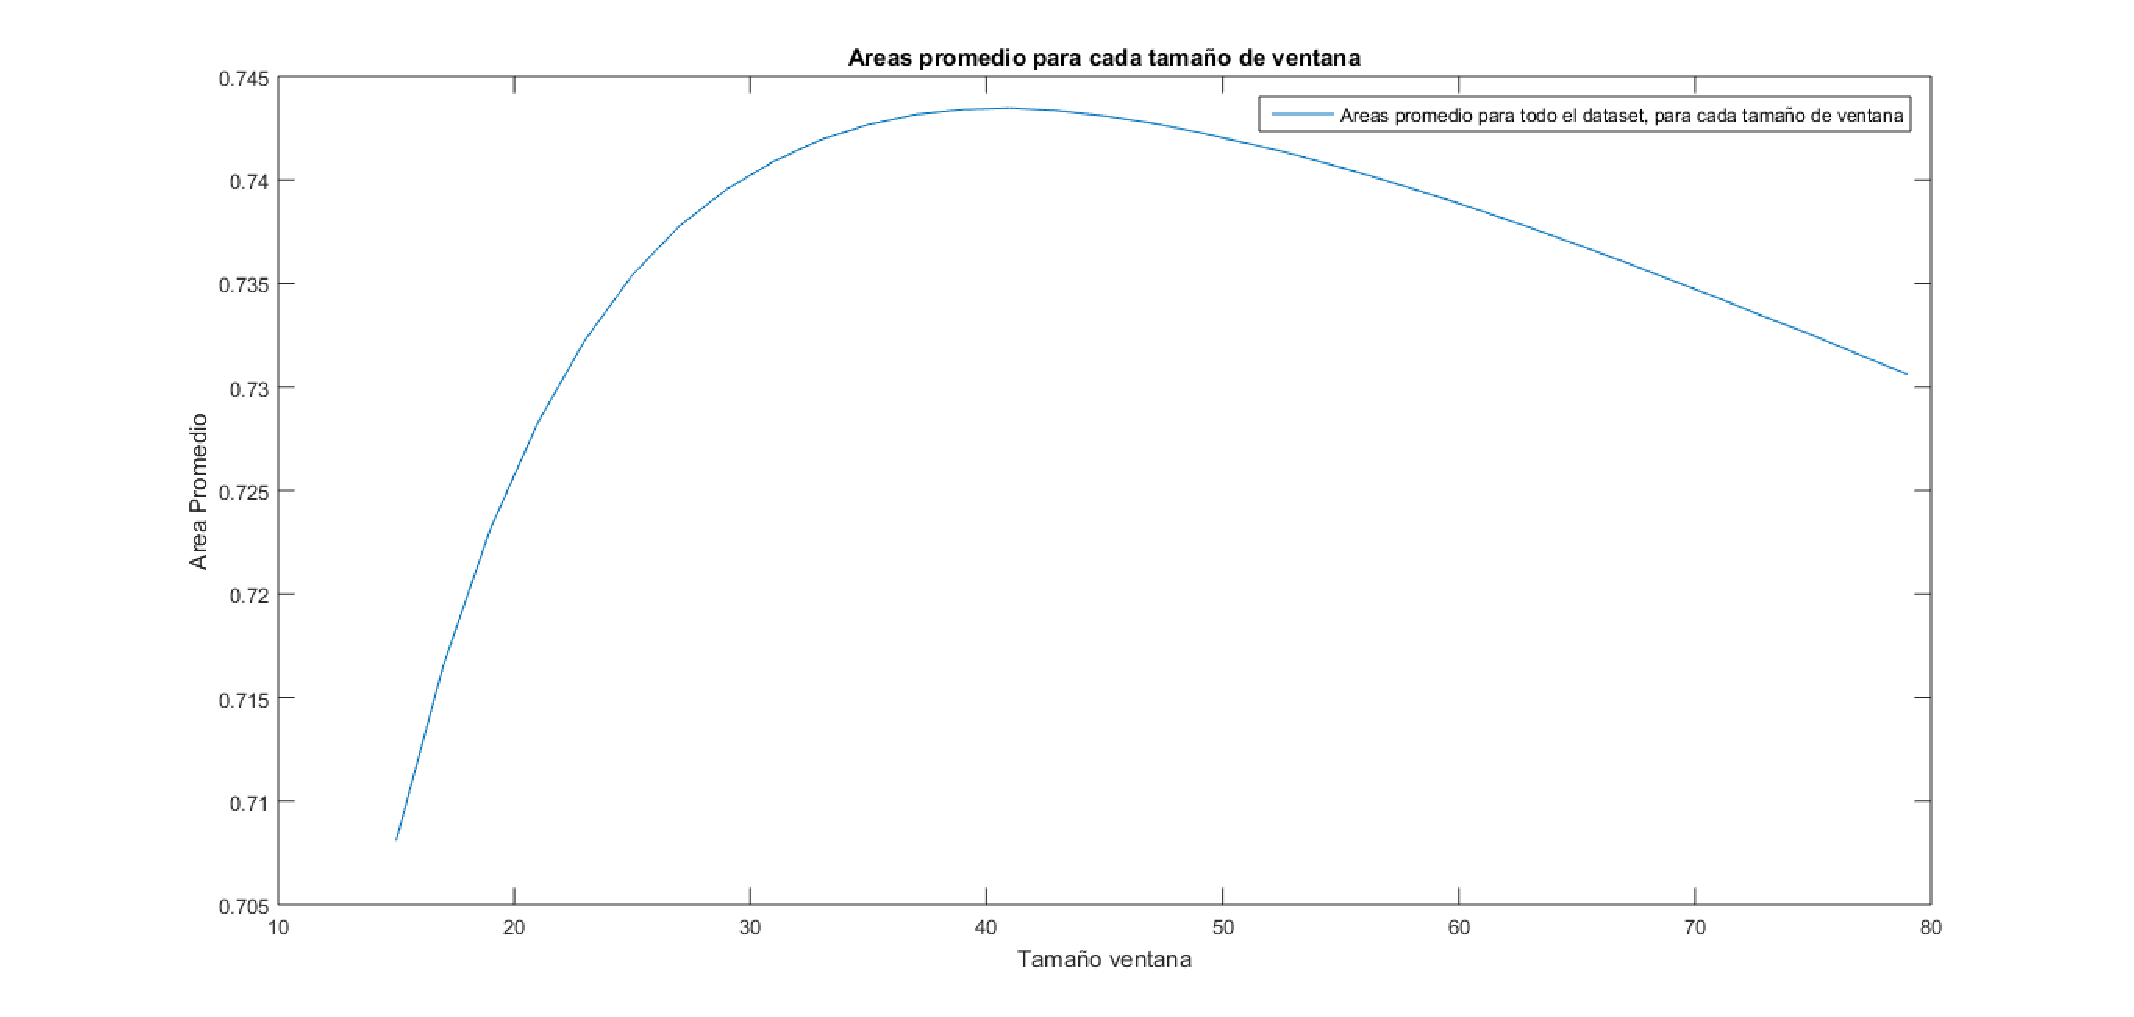
\includegraphics[width=1\textwidth]{Figures/MediaRangoChico}
	\caption[Ventana Media 15-80]{\'Areas promedio para diferentes tama\~nos de ventana, en el rango 15-80.}
	\label{fig:MediaRangoChico}
	}
\end{figure}

\begin{itemize}
	\item[$*$]Gaussiano
\end{itemize}

Para el filtro gaussiano no hay parámetros que varíen significativamente el resultado, por lo que solo se evaluó el resultado de aplicar el filtro con el mismo proceso mencionado para la media y mediana. 

A continuaci\'on se puede observar (\ref{fig:gaussiano}) que para las distintas imágenes no existe variación del resultado, y el área obtenida es 0.5469.


\begin{figure}[H]
	{
	\centering
	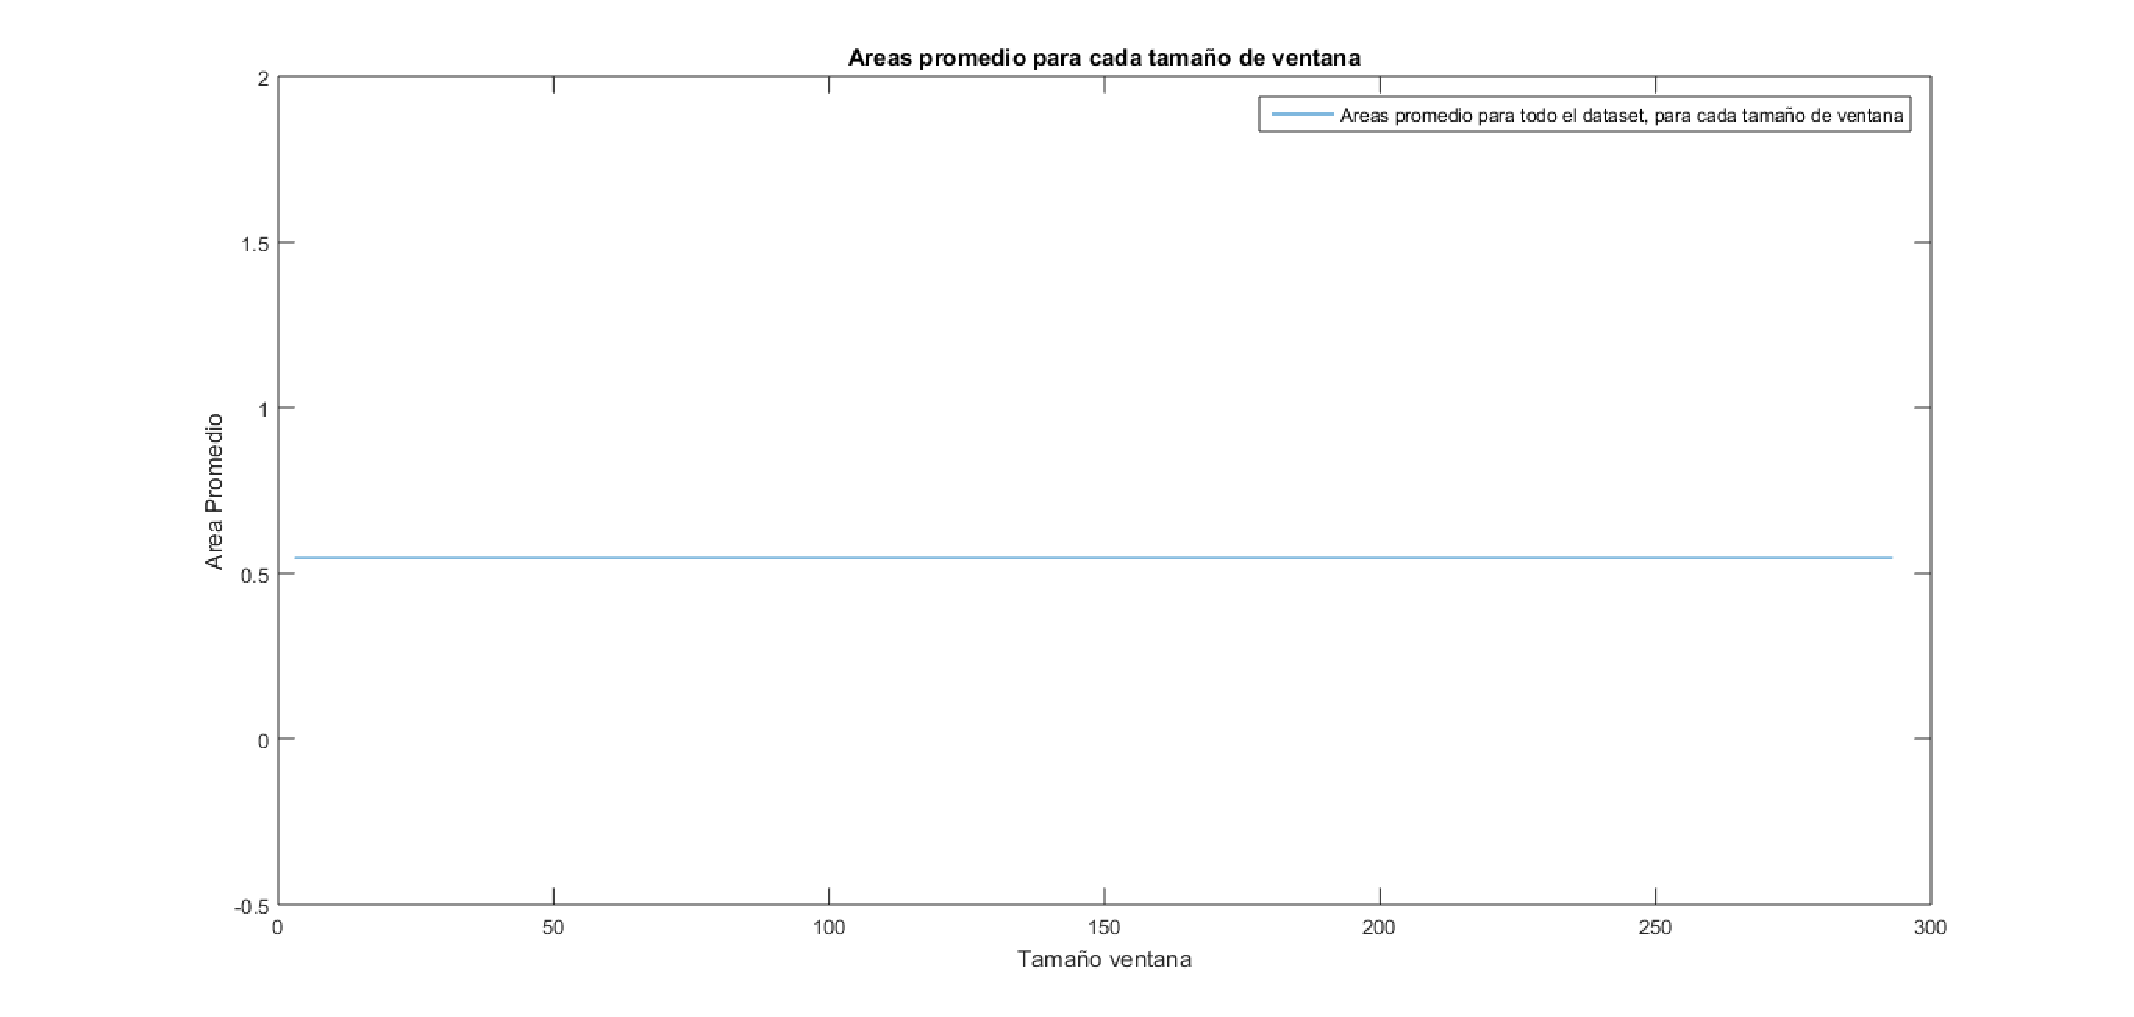
\includegraphics[width=1\textwidth]{Figures/Gaussiano}
	\caption[An Electron]{Areas promedio para cada imagen aplicando el filtro Gaussiano.}
	\label{fig:gaussiano}
	}
\end{figure}

Extracci\'on de ruido\\

En esta etapa se analiz\'o el mejor numero de iteraci\'on para los filtros de difusi\'on anisotr\'opica y filtro de coherencia en base a los resultados obtenidos. Para obtener un resultado \'optimo se realizaron iteraciones varias hasta encontrar el punto de inflexi\'on para este conjunto de im\'agenes.\\


\begin{itemize}
	\item[]Filtro de Difusi\'on Anisotr\'opica
\end{itemize}

Para las pruebas realizadas con este filtro se tuvo en cuenta la variaci\'on del parametro que hace referencia al n\'umero de iteraciones. Las mismas se variaron en un rango de entre 1 y 210 con pasos de 40,obteniendose de este modo, la gr\'afica siguinte (\ref{fig:anisotropica}):

\begin{figure}[H]
	{
	\centering
	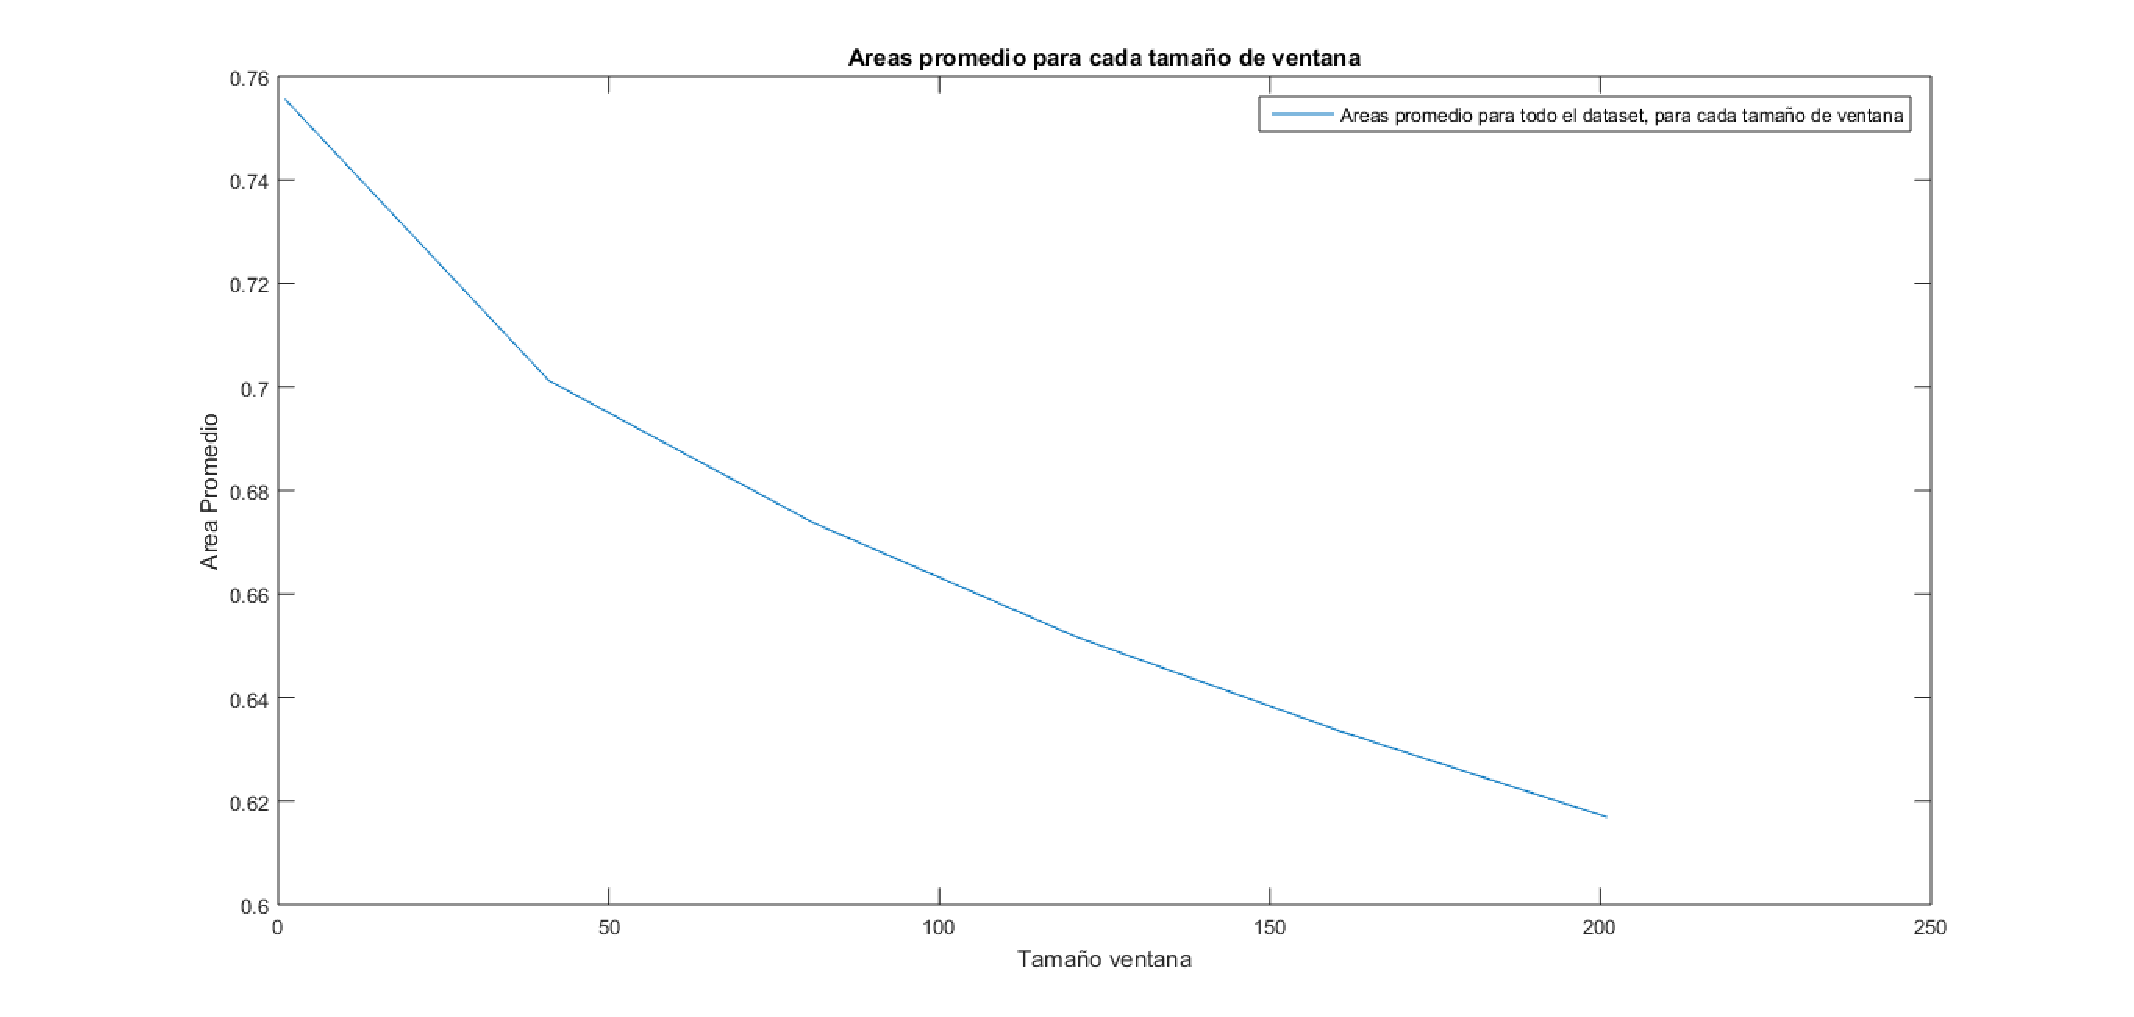
\includegraphics[width=1\textwidth]{Figures/AnisotropicoRangoGrande}
	\caption[An Electron]{Areas promedio para distintos valores de iteracion, en un rango 0-210.}
	\label{fig:anisotropica}
	}
\end{figure}

Con lo que se determino que los mejores resultados se obtienen entre los valores 1 y 50. Al repetir el proceso aplicando el filtro con cada valor de iteración entre el rango 1-50 se obtuvo:

\begin{figure}[H]
	{
	\centering
	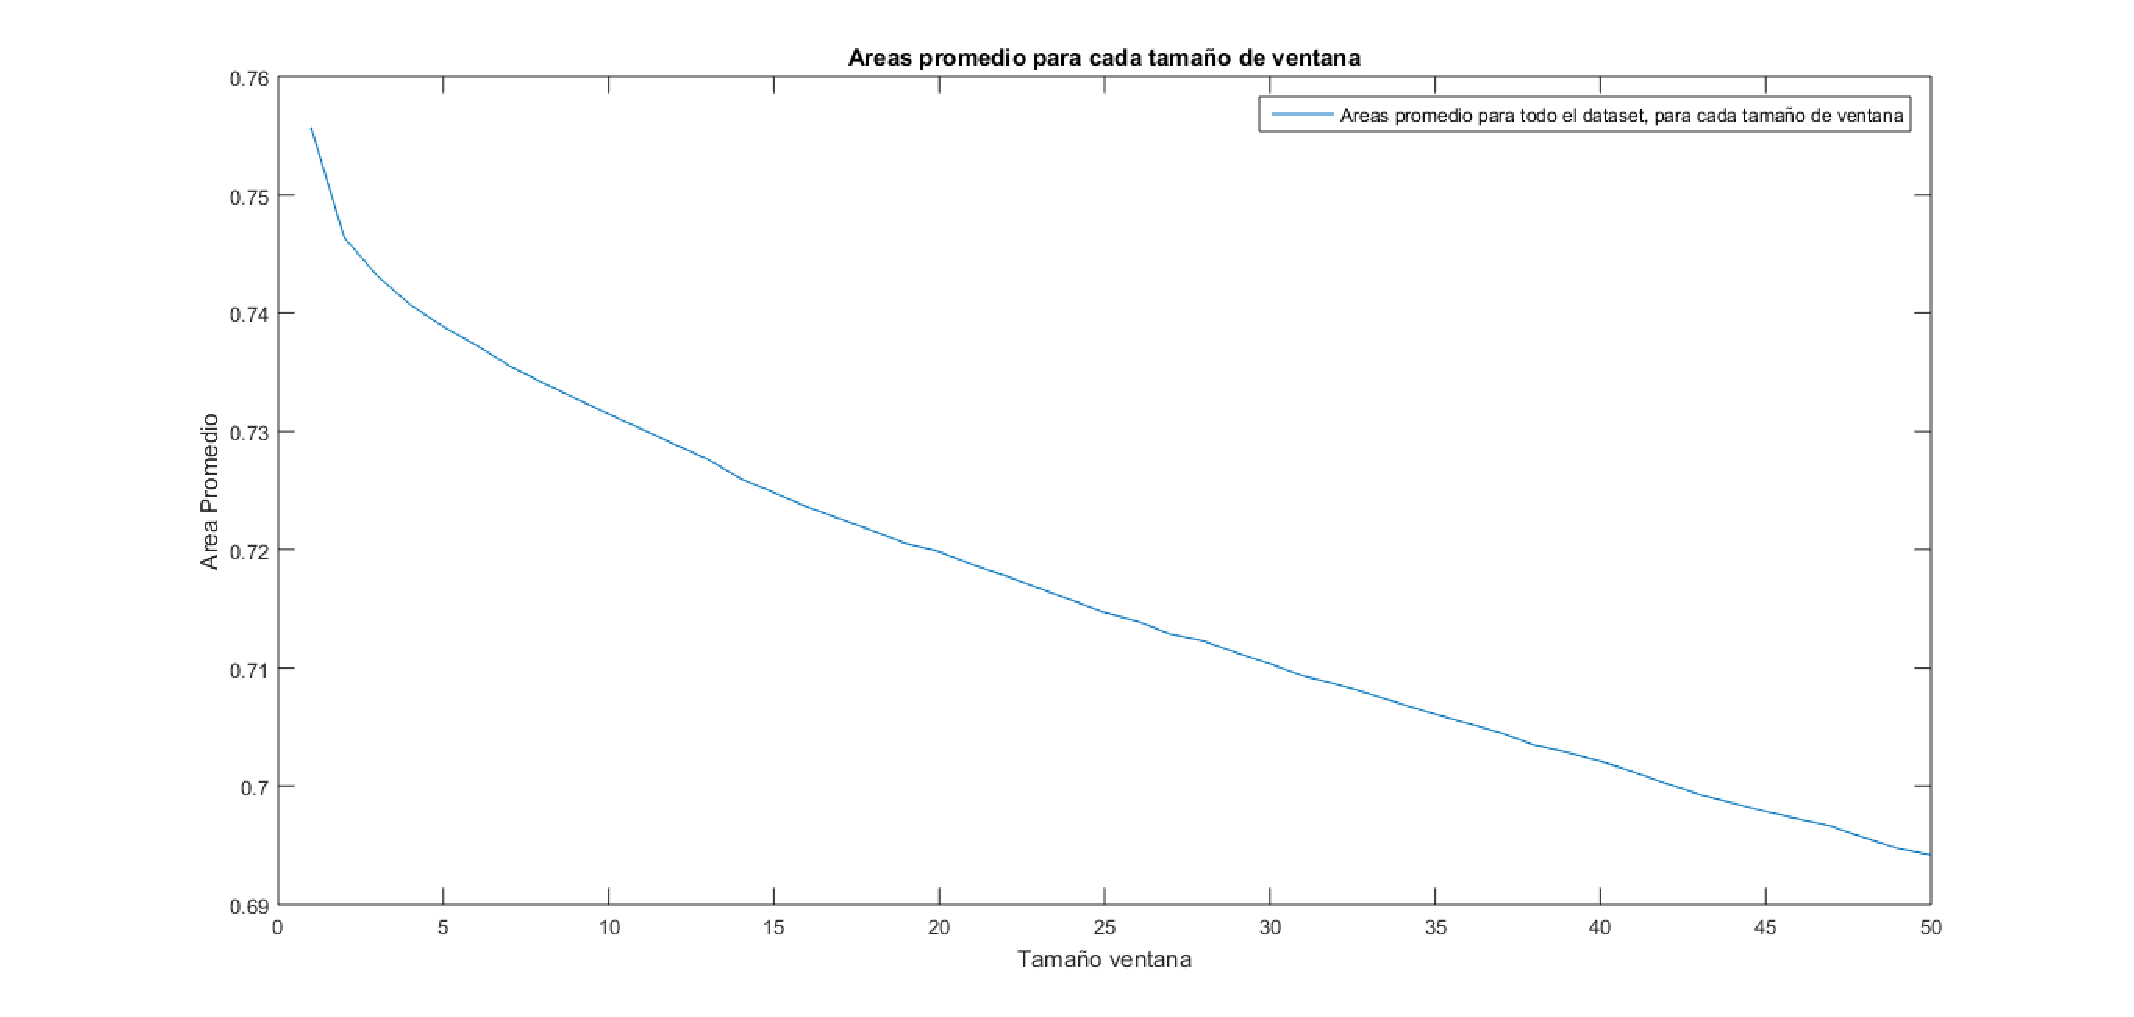
\includegraphics[width=1\textwidth]{Figures/AnisotropicoRangoChico}
	\caption[An Electron]{Areas promedio para distintos valores de iteracion, en un rango 1-50.}
	}
\end{figure}

Como podemos observar, el mejor resultado se obtuvo con la iteración 1 y un valor de  área promedio de 0.7557.

\begin{itemize}
	\item[]Filtro de Coherencia
\end{itemize}

El proceso para el filtro de coherencia se reali\'o de la misma forma que el de difusi\'on anisotr\'opica con iteraciones entre 3 y 450 con pasos de 50. Los resultados obtenidos fueron los siguientes (\ref{fig:coherencia}):

\begin{figure}[H]
	{
	\centering
	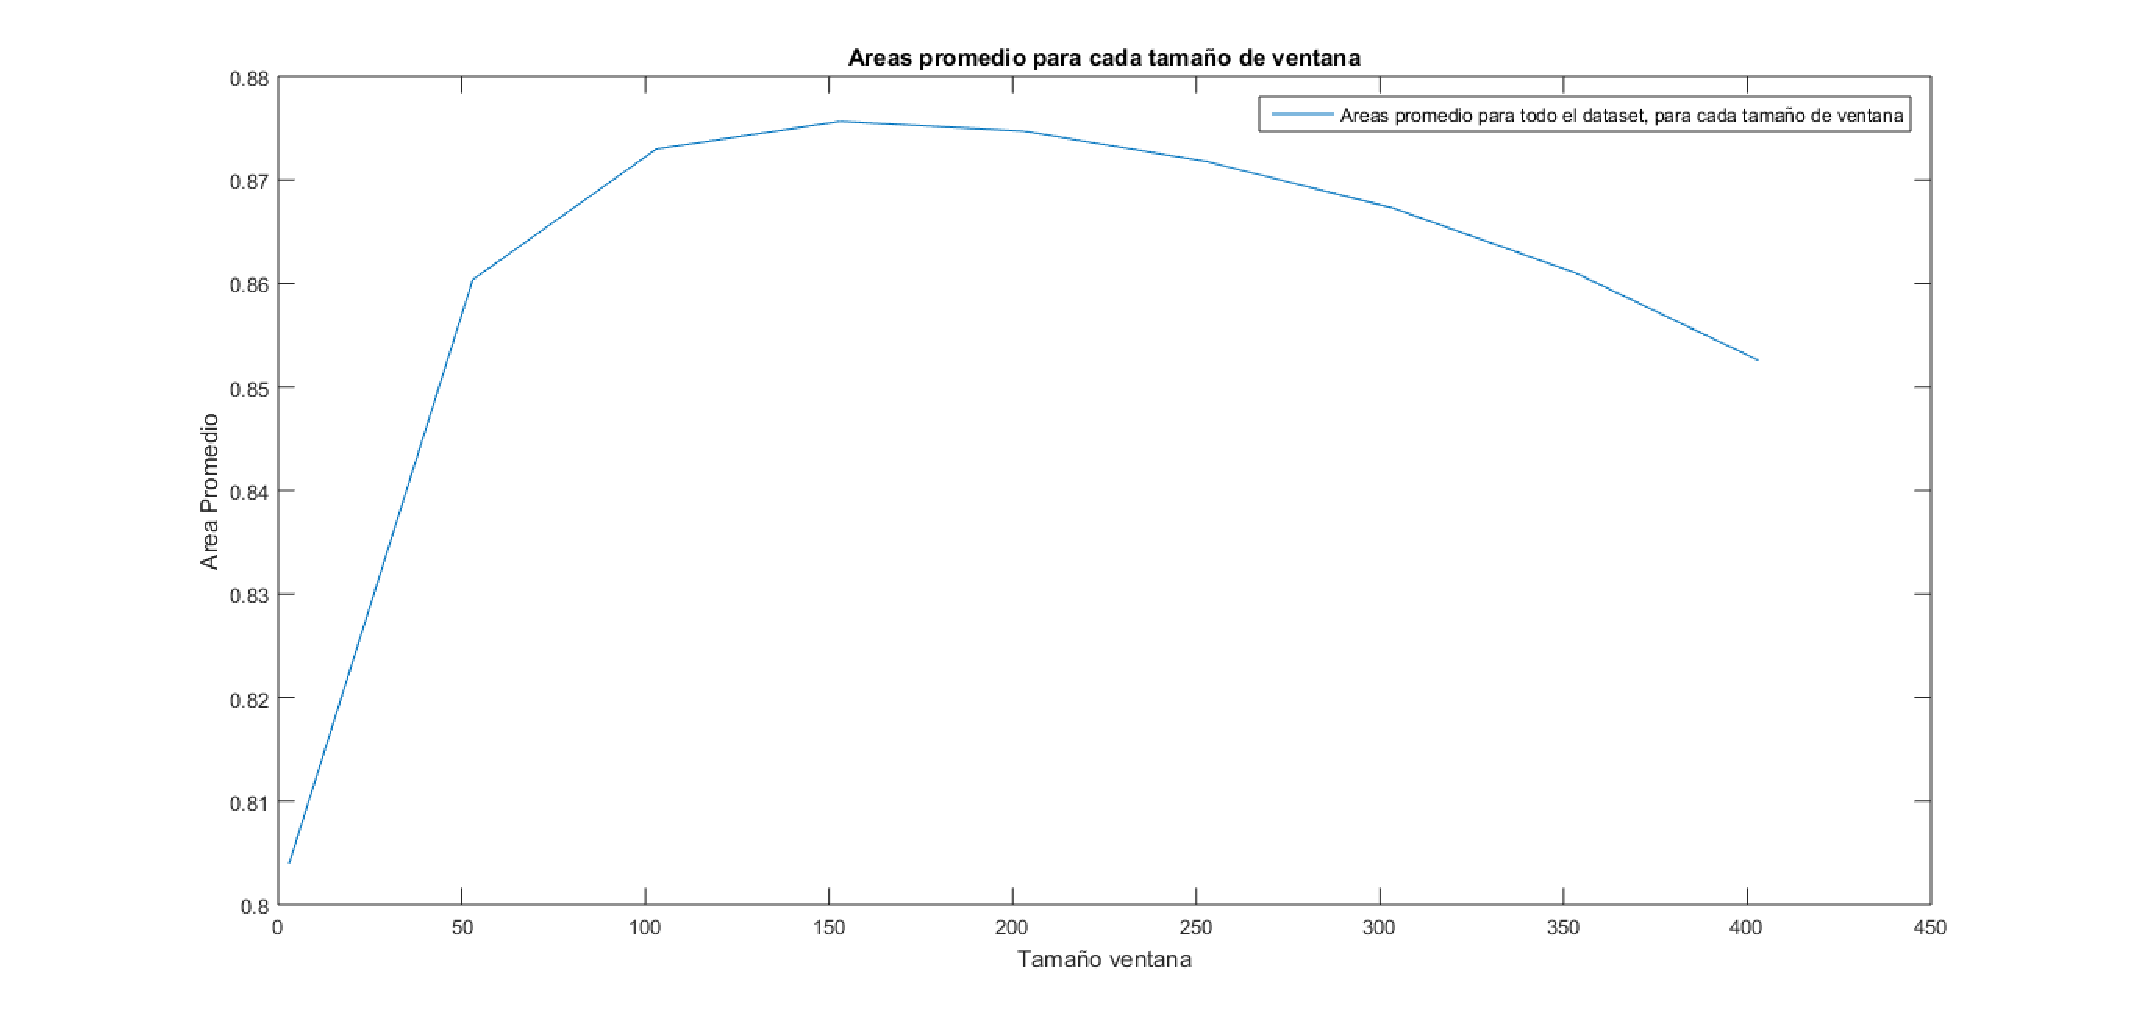
\includegraphics[width=1\textwidth]{Figures/CoherenciaRangoGrande}
	\caption[An Electron]{Areas promedio para distintos valores de iteracion, en un rango 0-550.}
	\label{fig:coherencia}
	}
\end{figure}

Observando el resultado se conluy\'o que los mejores resultados se obtienen con valores que iteran entre 140 y 160, por lo que se itero por cada uno de estos valores y se obtuvo (\ref{fig:coherenciaRangoChico}):

\begin{figure}[H]
	{
	\centering
	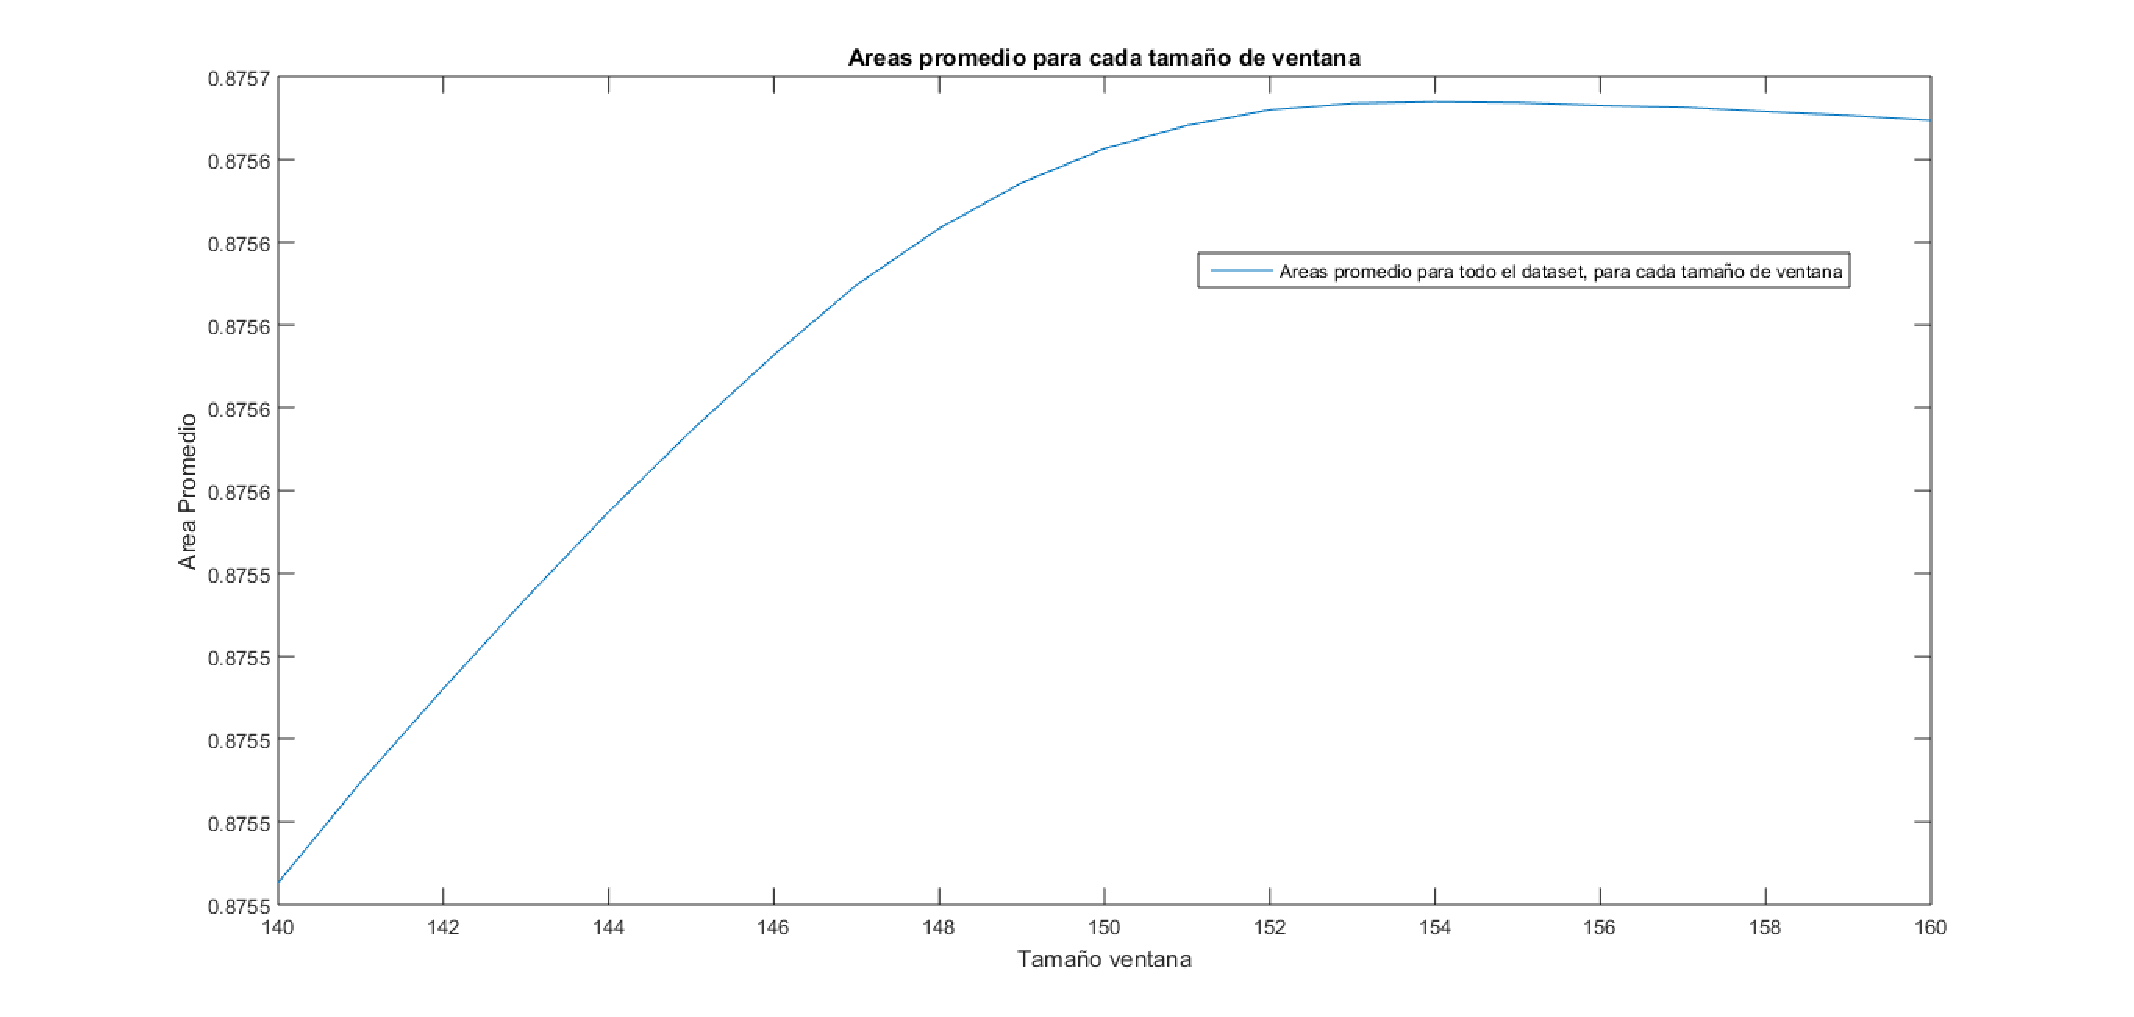
\includegraphics[width=1\textwidth]{Figures/CoherenciaRangoChico}
	\caption[An Electron]{Areas promedio para distintos valores de iteracion, en un rango 140-160.}
	\label{fig:coherenciaRangoChico}
	}
	\end{figure}

Finalmente se determin\'o que para el filtro de coherencia el parámetro de iteraciones consigue su valor \'optimo en 154 iteraciones, obteniendo un área de 0.8756 para este conjunto de im\'agenes.\\

A partir de este  \'analisis realizado en cada una de las etapas, se realizaron las pruebas de los pipeline definidos al principio. 


Como conclusi\'on podemos ver que en la fase de extracci\'on de fondo los mejores resultados se obtuvieron con la mediana, por tal raz\'on se utiliz\'o la misma para el objetivo de esta etapa con una ventana de 41x41. Para la fase de extracci\'on de ruido se observa que los mejores resultados se obtienen con el filtro de coherencia con 154 iteraciones. La etapa de realce simplemente utiliza la funci\'on adapthisteq que provee Matlab.\\




\subsection{Dataset HRF}

Para este conjunto de im\'agenes se utilizaron 3 tipos de im\'agenes, de las cuales 5 se corresponden con la enfermedad glaucoma, 5 con rentinopa\'ia diabetica y las restantes 5 son im\'agenes sanas. 

El proceso de las pruebas fue el mismo que se utiliz\'o para el dataset aria. Partiendo de una im\'agen con el canal verde, se realizaron las pruebas correspondientes a cada uno de los pipeline mencionados anteriormente, obteniendose los siguientes resultados.\\

Extracción de fondo
\begin{itemize}
	\item[$*$]Mediana 
\end{itemize}

En este caso para la obtenci\'on de la mejor ventana a utilizar en este dataset, se realiz\'o la b\'usqueda de la misma haciendo iteraciones que fueron desde 1 hasta 400 con pasos de 20. Finalizado esta prueba se obtuvo el siguiente resultado (\ref{fig:MedianaRangoGrandeHRF}): 

IMAGEN MEDIANA RANGO GRANDE

De la im\'agen anterior se puede ver que el punto m\'aximo de la par\'abola se encuentra en un rango menor, por tal raz\'on se realiza otra iteraci\'on en el rango X-Y con pasos de a 2. La im\'agen a continuaci\'on (\ref{fig:MedianaRangoChicoHRF}) nos muestra el resultado de la mejor ventana para la mediana, siendo esta 103.\\

IMAGEN MEDIANA RANGO CHICO

\begin{itemize}
	\item[$*$]Media
\end{itemize}

Para la b\'usqueda de la ventana \'optima en el caso de la media, se realiz\'o una iteraci\'on inicial que se encuentra en los valores de 1 a 400 con pasos de 20, observandose (\ref{fig:MediaRangoGrandeHRF}) que el valor \'optimo puede encontrarse en un rango mas pequeño, se realiz\'o la siguiente iteraci\'on con valores de entre X-Y con pasos de a 2. De esta forma se encontr\'o la mejor ventana, teniendo la misma un valor de 83.

IMAGEN MEDIA RANGO GRANDE Y CHICO

\begin{itemize}
	\item[$*$]Gaussiano
\end{itemize}

En el filtro gaussiano no hay parámetros que varíen significativamente el resultado, por lo que solo se evaluó el resultado de aplicar el filtro con el mismo proceso mencionado para la media y mediana.

IMAGEN GAUSSIANO


\begin{itemize}
	\item Pipeline 1
		\begin{itemize}
			\item	Extracci\'on de fondo (mediana) + Realce + Sacar Ruido (Anisotrópica): en este caso seutiliz\'o la la extracc se utilizó para 	sacar el ruido, la función anisotrópica con un valor de kappa=2 y número de iteraciones igual a 20, se obtuvo así un área promedio de 0.88634779241998385 para la iteración 1. Para valores mayores de kappa, disminuye el área promedio.
			\item	Sacar fondo (mediana) + Realce + Sacar Ruido (Coherencia): en este caso se realizaron 50 iteraciones, ya que en pruebas independientes se vio que a mayor número de iteraciones, mejores eran los resultados. El área promedio obtenida fue de 0.94650128394401889 para la iteración 50. Si bien el resultado aumenta hasta la iteración 105, no vale la pena llegar a tal punto ya que el aumento no es significativo con respecto al tiempo que tarda el algoritmo en realizar dichas iteraciones.
			\item Sacar fondo (media) + Realce + Sacar Ruido (Anisotrópica): en este caso se utilizó un kappa con valor igual a 2 y un número de iteraciones igual a 20. El área promedio obtenida fue de 	 	0.86863159426770764 para 20 iteraciones.
			\item Sacar fondo (media) + Realce + Sacar Ruido (Coherencia): se realizaron 50 iteraciones y se obtuvo un área promedio de 0.92994809994049088.
	\end{itemize}
	\item Pipeline 2
		\begin{itemize}
			\item Realce + Sacar Ruido (Anisotrópica): la función anisotrópica se realizó con 20 iteraciones para un valor de kappa igual a 2. El valor de área promedio obtenido fue de 0.3097178264596 para todas las iteraciones.
			\item	Realce + Sacar Ruido (Coherencia): la prueba se realizó con 50 iteraciones y se obtuvo un área promedio de  0.30937490250808752.
		\end{itemize}
	\item Pipeline 3
		\begin{itemize}
			\item Realce + Sacar fondo (mediana): En este caso se obtuvo un área promedio de 0.93866336888430779.
			\item Realce + Sacar fondo (media): en este caso se obtuvo un área promedio de 0.92444315570164037.
			\item Realce + Sacar fondo (Gaussiano): en este caso se obtuvo un área promedio de 0.48294301483035912. Como el valor obtenido es muy bajo respecto a los otros métodos utilizados para sacar el fondo, este método no se calculo más.
		\end{itemize}
	\item Pipeline 4
		\begin{itemize}
			\item Realce + Sacar fondo (media) + sacar ruido (anisotrópica): en este caso se obtuvo un área promedio de 0.89198264475071964, haciendo 20 iteraciones y con el valor de kappa igual a dos.
			\item Realce + Sacar fondo (mediana) + sacar ruido (anisotrópica): en este caso se obtuvo un área promedio de 0.896901101865378 con 20 iteraciones y el valor de kappa igual a dos.
			\item Realce + Sacar fondo (mediana) + sacar ruido (coherencia): en este caso, la prueba se realizó con 50 iteraciones y se obtuvo un área promedio de 0,9539922.
			\item Realce + Sacar fondo (media) + sacar ruido (coherencia): olvide hacer esta prueba, pero se ve en todos los casos que para sacar fondo, la mejor opción es la mediana.
		\end{itemize}
\end{itemize}


\subsection{Dataset DRIVE}


%-----------------------------------
%	SECTION 3
%-----------------------------------

\section{Extracci\'on de caracter\'isticas}


%----------------------------------------------------------------------------------------
%	SECTION 4
%----------------------------------------------------------------------------------------

\section{M\'etodo de segmentaci\'on}

